\chapter{Statistica descrittiva}

Il corso tratterà tre principali argomenti: \textbf{statistica descrittiva}, \textbf{probabilità} e
\textbf{inferenza statistica}.

Questa prima parte di \emph{statistica descrittiva} tratterà l'analisi di dati senza la costruzione di un
modello d'interpretazione.

Due dei concetti preliminari e fondamentali sono quelli di \textbf{popolazione} e \textbf{campione}:
\begin{itemize}
	\item \textbf{Popolazione}: cardinalità dell'insieme che stiamo considerando.
	\item \textbf{Campione}: cardinalità di un sottoinsieme più piccolo dell'insieme che stiamo considerando.
\end{itemize}

\begin{example}
	Gli italiani che hanno partecipato alle ultime votazioni (45 milioni circa) sono una \emph{popolazione}.
	Quando si fa un sondaggio elettorale si prende in considerazione un \emph{campione} della popolazione (per
	esempio qualche migliaio di votanti).
\end{example}

Altri due concetti di base sono quelli di \textbf{frequenza assoluta} e \textbf{frequenza relativa}:
\begin{itemize}
	\item \textbf{Frequenza assoluta}: il valore assoluto con il quale occorre un certo valore.
	\item \textbf{Frequenza relativa}: la percentuale con la quale un certo valore compare all'interno
	      dell'insieme dell'insieme considerato.
\end{itemize}

\begin{example}
	Se un candidato sindaco prende 1234 voti su 6342 votanti allora 1234 è la \emph{frequenza assoluta} del
	suo voto. La frequenza relativa si calcola banalmente:
	\[ \frac{1234}{6342} = 0.194 \]
	dunque $0.194$ è la \emph{frequenza relativa} del voto, ossia il $19.4 \%$ dei voti.
\end{example}

\section{Rappresentazione grafica delle frequenze}
In statistica si farà spesso uso di rappresentazioni grafiche di vario genere come diagrammi a torta, istogrammi, grafici
di dispersione ecc.
\begin{figure}[!h]
	\centering
	\caption*{Diagramma a torta}
	\begin{tikzpicture}[scale=0.7]
		\pie[text=inside, color = { yellow!60, red!60, blue!60 }] {
			40/Giallo,
			25/Rosso,
			45/Blu
		}
	\end{tikzpicture}
\end{figure}

\begin{center}
	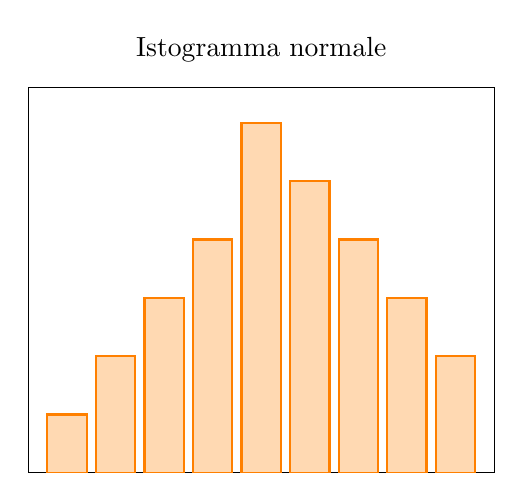
\begin{tikzpicture}
		\begin{axis}[
				title={Istogramma normale},
				xtick=\empty,
				ytick=\empty,
				ymin=0,
				width=7.5cm,
				ybar,
				bar width=0.5cm,
				grid=both,
				grid style=dashed
			]

			\addplot [
				thick,
				draw=orange,
				fill=orange!30,
			]
			coordinates {(0, 1) (1, 2) (2, 3) (3, 4) (4, 6) (5, 5) (6, 4) (7, 3) (8, 2)};
		\end{axis}
	\end{tikzpicture}
	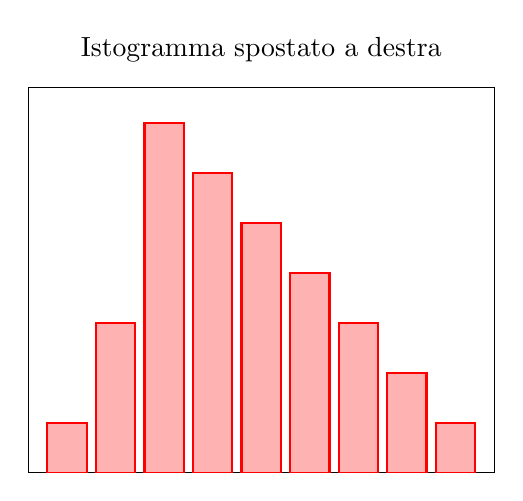
\begin{tikzpicture}
		\begin{axis}[
				title={Istogramma spostato a destra},
				xtick=\empty,
				ytick=\empty,
				ymin=0,
				width=7.5cm,
				ybar,
				bar width=0.5cm,
				grid=both,
				grid style=dashed
			]
			\addplot [
				thick,
				draw=red,
				fill=red!30,
			] coordinates {(0, 1) (1, 3) (2, 7) (3, 6) (4, 5) (5, 4) (6, 3) (7, 2) (8, 1)};
		\end{axis}
	\end{tikzpicture}

	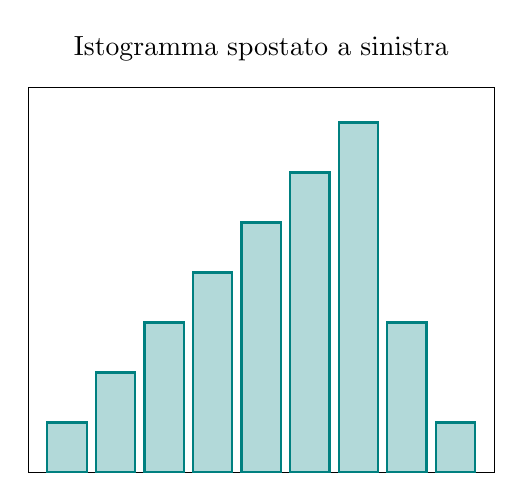
\begin{tikzpicture}
		\begin{axis}[
				title={Istogramma spostato a sinistra},
				xtick=\empty,
				ytick=\empty,
				ymin=0,
				width=7.5cm,
				ybar,
				bar width=0.5cm,
				grid=both,
				grid style=dashed
			]

			\addplot [
				thick,
				draw=teal,
				fill=teal!30,
			]
			coordinates {(0, 1) (1, 2) (2, 3) (3, 4) (4, 5) (5, 6) (6, 7) (7, 3) (8, 1)};
		\end{axis}
	\end{tikzpicture}
	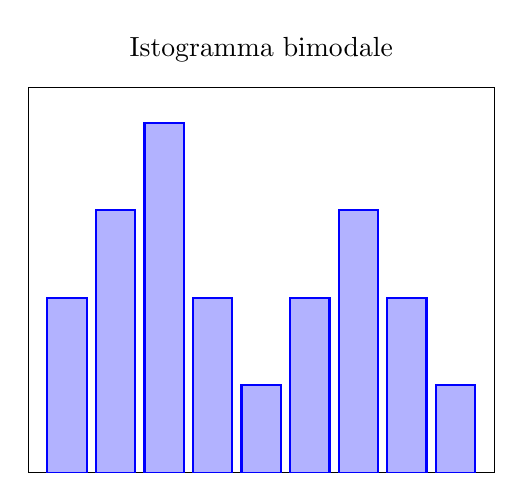
\begin{tikzpicture}
		\begin{axis}[
				title={Istogramma bimodale},
				xtick=\empty,
				ytick=\empty,
				ymin=0,
				width=7.5cm,
				ybar,
				bar width=0.5cm,
				grid=both,
				grid style=dashed
			]
			\addplot [
				thick,
				draw=blue,
				fill=blue!30
			]
			coordinates {(0, 2) (1, 3) (2, 4) (3, 2) (4, 1) (5, 2) (6, 3) (7, 2) (8, 1)};
		\end{axis}
	\end{tikzpicture}
\end{center}

\section{Analisi di dati numerici}
Procediamo con alcune definizioni fondamentali per l'analisi statistica dei dati.

\begin{definition} \label{vettore}
	Definiamo \textbf{vettore di dati}, un insieme di valori, potenzialmente tutti diversi.
	\[ x = (x_1, x_2, \dots, x_n) \]
\end{definition}

\begin{definition}
	Definiamo la \textbf{media empirica} o il \textbf{valore medio} come la media aritmetica dei valori in un certo
	vettore di dati.
	\[ \overline{x} = \frac{x_1 + x_2 + \dots + x_n}{n} \]
\end{definition}

\subsection{Varianza}
La \textbf{varianza} è il valore che definisce la \emph{variabilità} di un campione o meglio è una misura di
\emph{dispersione} dei dati. Andremo a vedere due tipi di varianza: campionaria ed empirica.

\begin{definition}
	Sia $x$ un vettore di dati, definiamo la \textbf{varianza campionaria} come segue:
	\[ \Var(x) = \sum_{i=1}^n \frac{(x_i - \overline{x})^2}{n - 1} \]
\end{definition}

\begin{definition}
	Sia $x$ un vettore di dati, definiamo la \textbf{varianza empirica} come segue:
	\[ \Var_e(x) = \sum_{i=1}^n \frac{(x_i - \overline{x})^2}{n} \]
\end{definition}

Non andremo ad analizzare perché la varianza sia definita in questo modo, per il momento ci basti sapere che:
\begin{itemize}
	\item La varianza campionaria si applica meglio ai campioni.
	\item La varianza empirica si applica meglio alle popolazioni.
\end{itemize}

\begin{observation}
	Se andiamo ad analizzare entrambe le formule possiamo facilmente accorgerci che la varianza, essendo una somma di
	quadrati, ha valore 0, quando questi sono tutti 0. Perché questo avvenga, tutti i valori in $x$ devono essere
	uguali fra di loro.

	Ecco che possiamo dire che un valore basso di varianza corrisponde ad un vettore di dati con valori molto simili
	fra loro. Al contrario, un alto valore di varianza corrisponde ad un vettore di dati con valori molto diversi fra
	loro.

	Presi due vettori di dati differenti, uno con valori molto simili fra loro e uno con valori molto diversi. La
	media potrebbe essere molto simile se non uguale ma la varianza per i due vettori sarà differente.
\end{observation}

\begin{definition}

	Definiamo anche un'uguaglianza di base che, per il momento non andremo a spiegare, ma che in seguito ci tornerà
	utile:
	\[ \sum_{i=1}^n (x_i - \overline{x})^2 = \sum_{i=1}^n x_i^2 - n \overline{x}^2 \]
	\begin{proof}
		Sviluppando il quadrato possiamo facilmente convincerci che l'uguaglianza sia vera:
		\[
			\begin{array}{ l l l l }
				  & \displaystyle\sum_{i=1}^n (x_i - \overline{x})^2                                     & = &
				\displaystyle\sum_{i=1}^n (x_i^2 - 2x_i \overline{x} + \overline{x}^2)                         \\
				\\
				= & \displaystyle\sum_{i=1}^n x_i^2 - 2 \overline{x} \sum_{i=1}^n x_i + n \overline{x}^2 &
				= & \displaystyle\sum_{i=1}^n x_i^2 - 2 n \overline{x}^2 + n \overline{x}^2                    \\
				\\
				= & \displaystyle\sum_{i=1}^n x_i^2 - n \overline{x}^2
			\end{array}
		\]
	\end{proof}
\end{definition}

\begin{definition}
	Definiamo lo \textbf{scarto quadratico medio} come la radice quadrata della varianza campionaria:
	\[ \sigma (x) = \sqrt{\Var (x)} \]
\end{definition}

\begin{definition}
	Definiamo la \textbf{deviazione standard} come la radice quadrata della varianza empirica:
	\[ \sigma_e (x) = \sqrt{\Var_e (x)} \]
\end{definition}

Come già detto in precendenza, la varianza è nulla se e solo se tutti i valori nel vettore $x$ sono uguali tra di loro,
vale quindi
\[ \Var(x) = 0 \Leftrightarrow x_1 = x_2 = \dots = x_n \]
Abbiamo anche già specificato che il valore della varianza indica il grado di \emph{dispersione} dei dati, per fissare
meglio il concetto analizziamo questa espressione:
\[ \# \{ x_i : |x_i - \overline{x}| > d  \} \leq \frac{\displaystyle\sum_{i=1}^n (x_i - \overline{x})}{d^2} \]
Da qui possiamo dedurre che
\[ \frac{\# \{ x_i : |x_i - \overline{x}| > d \}}{n} \leq \frac{\Var_e(x)}{d^2} \]
La disequazione appena descritta è detta \textbf{disuguaglianza di Chebyshev}, anche se, come vedremo più avanti, si
tratta di un caso particolare della vera disuguaglianza di Chebyshev. Essa indica la percentuale di dati che differiscono
da $\overline{x}$ per almeno un fattore $d$.

\begin{observation}
	Questo ci dice che più la varianza è piccola, più diminuisce la percentuale di dati che differiscono dalla media per
	almeno un fattore $d$.
\end{observation}